\documentclass[9pt]{beamer}
\usepackage[ruled, french, onelanguage]{algorithm2e}
\usepackage{tikz}
\usepackage{listings}
\usepackage{hyperref}
\usepackage{amsmath}
\usepackage{amssymb}
\usepackage{xcolor}

\usetheme{Rochester}
\usecolortheme{default}

\title[exposé]{Deep learning pour la résolution de la MHD}
\author[V. Italiano]{Vincent Italiano}

\begin{document}
\begin{frame}    
    \maketitle

\end{frame}

\begin{frame}
    \frametitle{Objectifs du stage}

    On considère des EDP du type 

    $$
    \begin{cases}
        \partial_t u = \mathcal{L}(u, \partial_x u, \partial_{xx}u, \dots, \alpha) \\
        u(0,x) = u_0(x) \\
        u = u_b \text{ sur le bord }
    \end{cases}
    $$
    avec $\alpha\in V$ un paramètre.\\
    \vspace{1cm}

    but : construire des modèle réduit

\end{frame}

\begin{frame}
    \frametitle{Physics-Informed-Neural-Networks (PINNs)}

    \begin{center}
        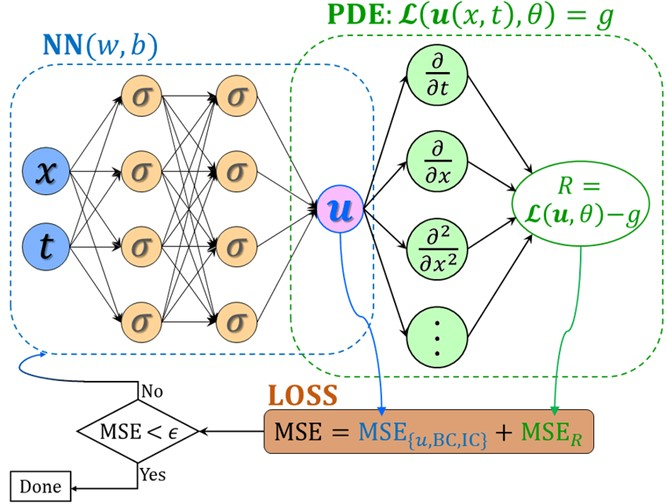
\includegraphics[scale=0.5]{img/pinns.jpg}
    \end{center}

\end{frame}

\begin{frame}
    \frametitle{Physics-Informed-Neural-Networks (PINNs)}
    \small Loss donnée par
    $$
    J_\theta(X) :=J_\theta^r(X^r) +J_\theta^0(X^0) + J_\theta^b(X^b)
$$
\begin{itemize}
    \item MSE sur le résidu 
    $$
   J_\theta^r(X^r) = \frac{1}{N_r}\sum_{i=1}^{N_r} \left|r_\theta\left(t_i^r, x_i^r\right)\right|^2
    $$
avec $X^r:=\{(t_i^r, x_i^r)\}_{i=1}^{N_r} \subset ]0,T] \times \mathcal{D}$, et $r_\theta$ est le résidu de l'EDP
    \item MSE sur les conditions initiale et conditions au bord
    $$
       J_\theta^0(X^0) 
       = 
       \frac{1}{N_0}
       \sum_{i=1}^{N_0} \left|u_\theta\left(t_i^0, x_i^0\right) - u_0\left(x_i^0\right)\right|^2
    $$ et $$
       J_\theta^b(X^b) 
       = 
       \frac{1}{N_b}
       \sum_{i=1}^{N_b} \left|u_\theta\left(t_i^b, x_i^b\right) - u_b\left(t_i^b, x_i^b\right)\right|^2
    $$
    où $X^0:=\{(t^0_i,x^0_i)\}_{i=1}^{N_0} \subset \{0\} \times \mathcal{D}$ et $X^b:=\{(t^b_i,x^b_i)\}_{i=1}^{N_b} \subset ]0,T] \times \partial \mathcal{D}$, 
    et  $u_\theta$ est le PINN.
\end{itemize}
\end{frame}

\begin{frame}
    \frametitle{Roadmap}

    \begin{itemize}
        \item Comprehension et prise en main d'un code PINN. \textcolor{green}{\checkmark}
        \item Essais sur l'équations de burgers en 1D. \textcolor{green}{\checkmark}
        \item Implémenter l'échantillonage préférentiel. \textcolor{green}{\checkmark}
        \item Réduction de modèle sur l'équation de Burgers. \textcolor{green}{\checkmark}
        \item Faire un cas en 2D. \textcolor{green}{\checkmark}
        \item Compréhension et implémentation de la MHD réduite. \textcolor{green}{\checkmark}
        \item Résolution de la MHD avec des PINNs.
        \item Réduction de modèle sur la MHD.
    \end{itemize}
\end{frame}

\begin{frame}
    \frametitle{Equation de Burgers en 1D}

    1er cas test : $\Omega = [0,1]\times[-1,1]$ et un paramètre de viscosité $\nu$

    $$
    \begin{cases}
        \partial_t u + \frac{1}{2}\partial_x u^2 = \nu \partial_{xx}u \quad \text{ sur } \Omega\\
        u(0,x) = \sin(\pi x) \quad \forall x \in [-1,1]\\
        u(t,-1) = u(t,1) = 0 \quad \forall t \in [0,1]
    \end{cases}
    $$
  
\end{frame}

\begin{frame}
    \frametitle{Premier résultats numérique : $\nu  =3\times 10^{-3}$}
    Avec un réseaux de taille 8x20, après 10min d'entrainements
    \begin{center}
        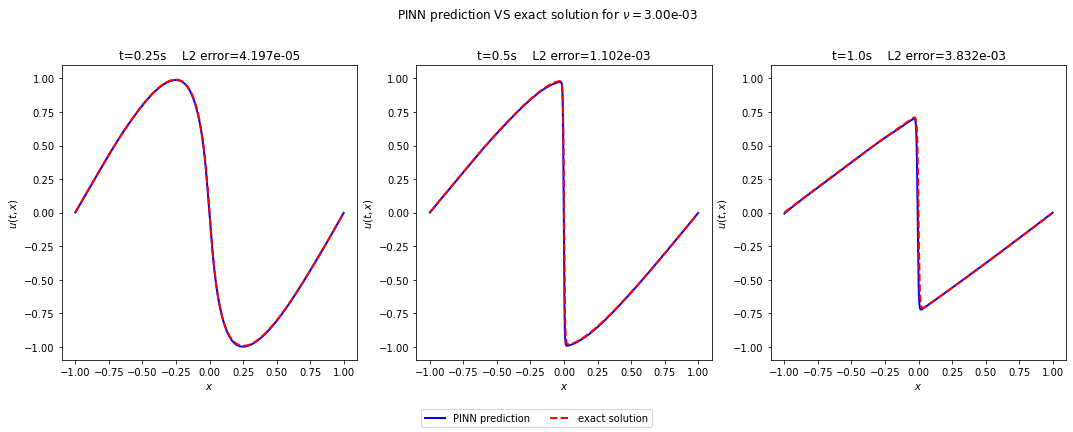
\includegraphics[width=1.\textwidth, height=0.3\textwidth]{img/burgers_nu1.png}
        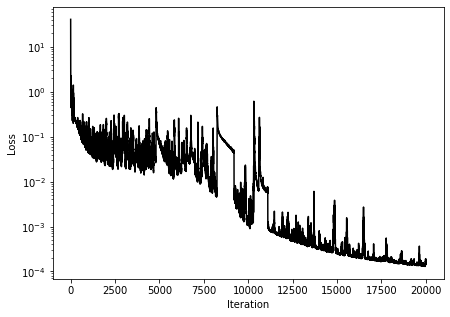
\includegraphics[width=0.49\textwidth,height=0.3\textwidth]{img/burgers_loss1.png}
        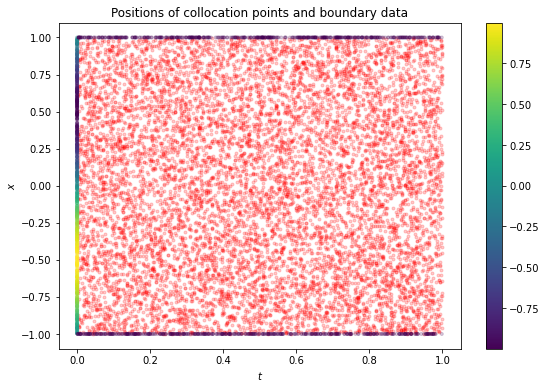
\includegraphics[width=0.49\textwidth,height=0.3\textwidth]{img/burgers_data.png}
    \end{center}

\end{frame}

\begin{frame}
    \frametitle{Echantillonage préférentiel}

    idée : modifier le tirage des points pour l'entrainements pour accélérer la convergence.

    \begin{itemize}
        \item En utilisant le résidu : on choisi les points ou le résidu est le plus grand.
        
        \item En utilisant un critère physique (l'entropie par ex) : on choisi les points ou l'entropie est la plus grande.
    \end{itemize}
\vspace*{1cm}
\begin{center}
    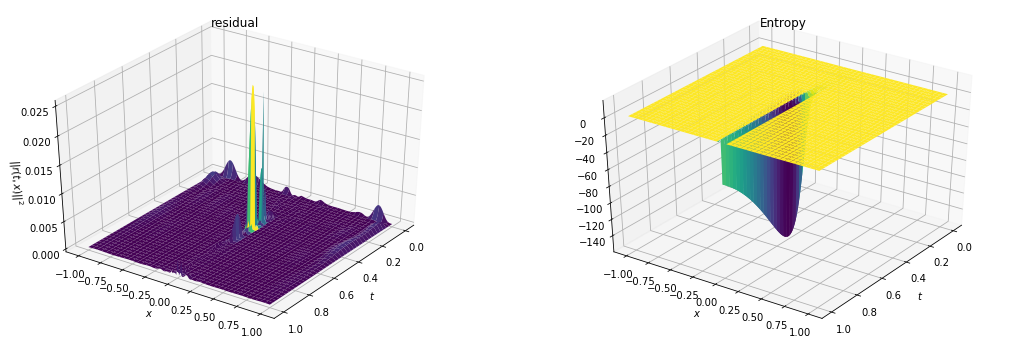
\includegraphics[width=1.\textwidth, height=0.3\textwidth]{img/adaptatif.png}
\end{center}
\end{frame}


\begin{frame}
    \begin{algorithm}[H]
        \KwData{Le reseau $u_{\theta}$, taille de batch $m$, ratio de points tiré uniformément $\alpha$}
        Générer $N$ points de collocation tiré uniformément\\
        Initialiser le reseau avec les paramètres $\theta^{(0)}$\\
        \While{$J(\theta^{(i)})>\varepsilon$}{
            Calculer la loss sur chaque points\\
            Calculer les $q_j^{(i)}$ selon le critère choisi\\
            Tirer $(1-\alpha) m$ points de collocation selon la loi multinomiale de paramètre $p^{(i)}=(q_j^{(i)})$\\
            Tirer $\alpha m$ points de collocation selon la loi uniforme.\\
            Effectuer la descente de gradient sur le batch obtenu.\\
        }
        \caption{Echantillonage préférentiel}
    \end{algorithm}

    avec le résidu :  $q_j^{(i)} = \frac{J(\theta^{(i)}, x_j)}{\sum_{j=1}^N J(\theta^{(i)}, x_j)}$, avec l'entropie : $q_j^{(i)} = \frac{S^2(\theta^{(i)}, x_j)}{\sum_{j=1}^N S^2(\theta^{(i)}, x_j)}$
    
\end{frame}

\begin{frame}

    Le temps d'entrainement avec un échantillonage préférentiel est plus long (evaluation de la loss en chaque points) 
    mais permet de converger plus vite (en itérations).\\
    \begin{center}
        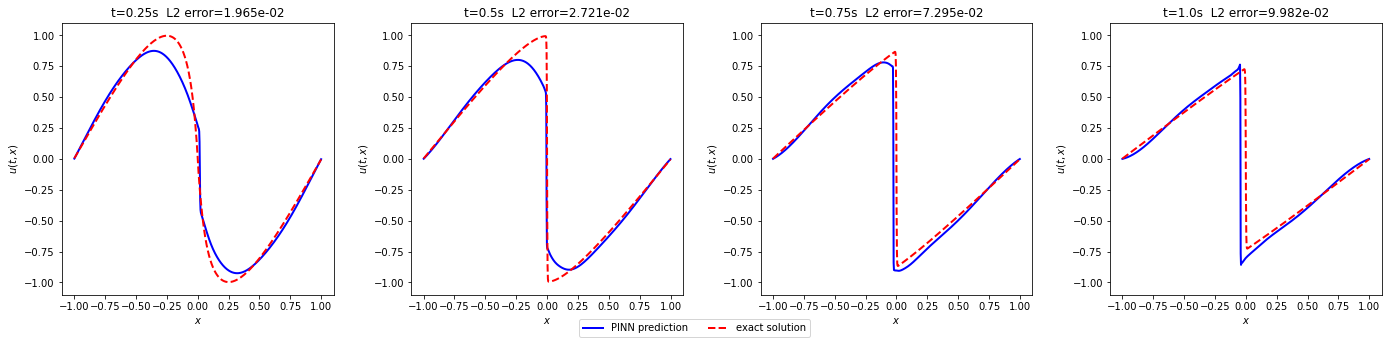
\includegraphics[width=.7\textwidth, height=0.4\textwidth, keepaspectratio]{img/adapt_uniforme1.png}
        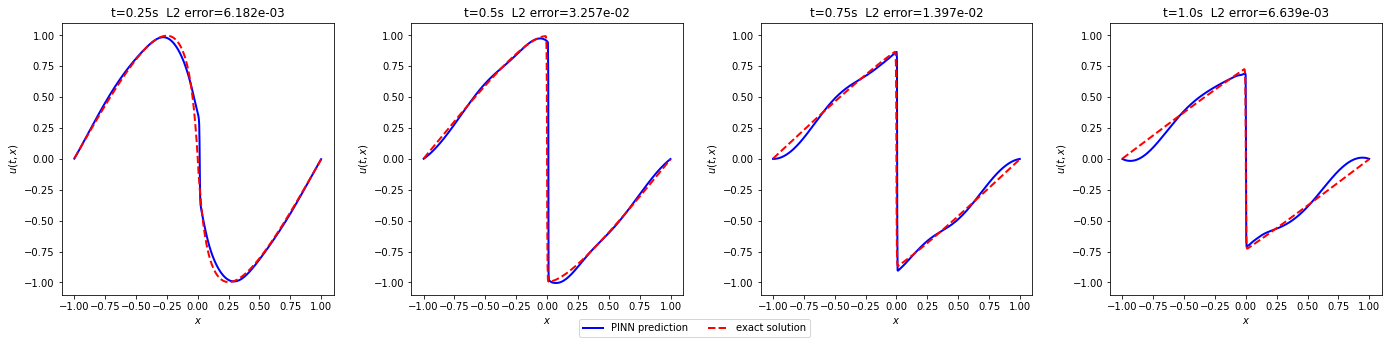
\includegraphics[width=.7\textwidth, height=0.4\textwidth, keepaspectratio]{img/adapt_residu1.png}
    \end{center}
    \tiny haut : uniforme.  bas : résidu\\
    \vspace*{1cm} 
    \normalsize Il devient inutile lorsqu'on a beaucoup de points de collocations.
\end{frame}

\begin{frame}
    \frametitle{Multiple viscosité}
    \begin{columns}
        \begin{column}{0.4\textwidth}

            \small Idée : la viscosité devient une variable $\to$ problème 3D.\\

             
            \begin{itemize}
                \item Réseau de taille 16x256
                \item 2h d'entrainements
                \item Plage de viscosité allant de $10^{-2}$ à $10^{-4}$
                \item Loss finale : $10^{-5}$
            \end{itemize}
        \end{column}
        \begin{column}{0.6\textwidth}  %%<--- here
            \vspace{-0.5cm}
            \begin{center}
                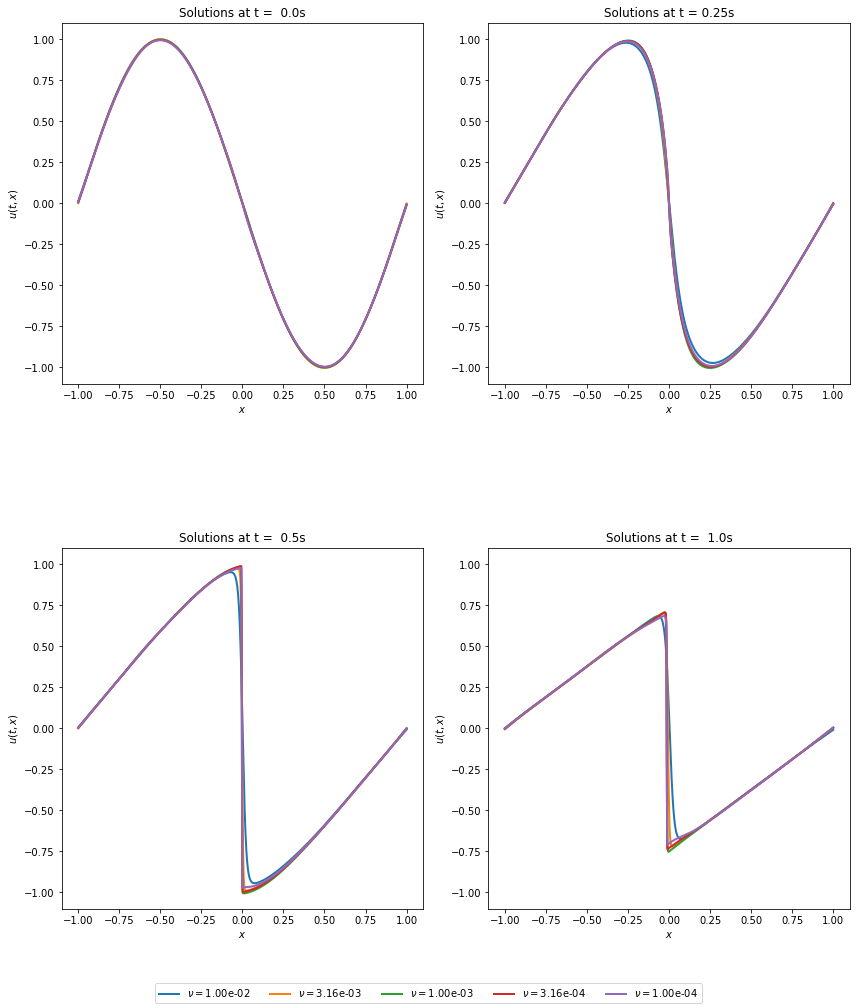
\includegraphics[scale=0.2]{img/burgers_bg.png}
             \end{center}
        \end{column}
        \end{columns}

\end{frame}

\begin{frame}

    \begin{center}
        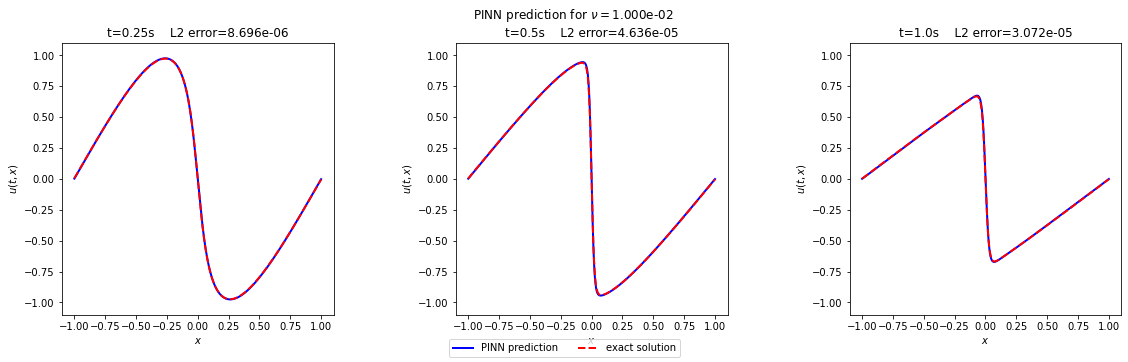
\includegraphics[width=.49\textwidth, height=0.4\textwidth, keepaspectratio]{img/burgers_multi1.png}
        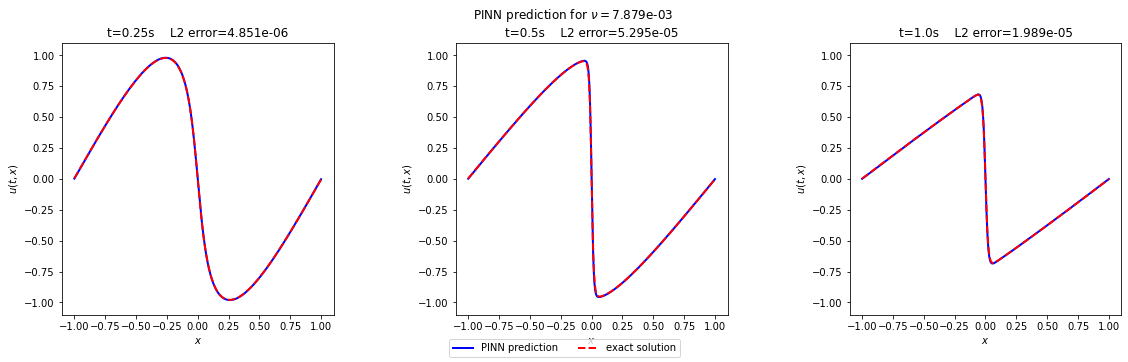
\includegraphics[width=.49\textwidth, height=0.4\textwidth, keepaspectratio]{img/burgers_multi2.png}
        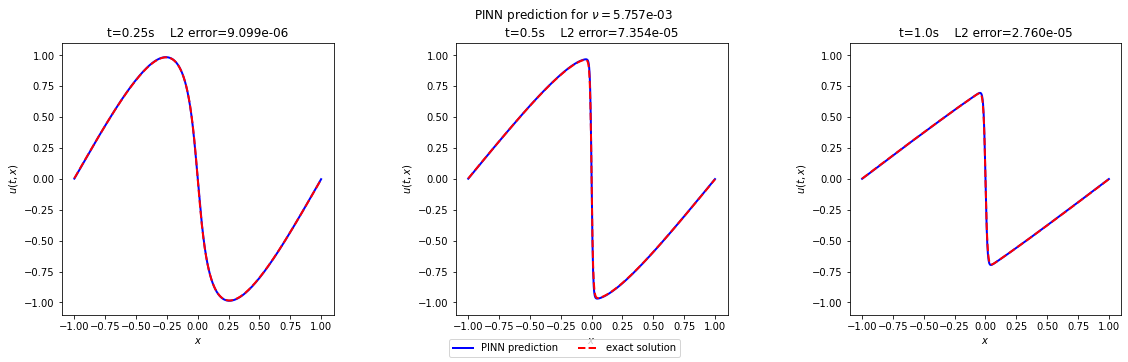
\includegraphics[width=.49\textwidth, height=0.4\textwidth, keepaspectratio]{img/burgers_multi3.png}
        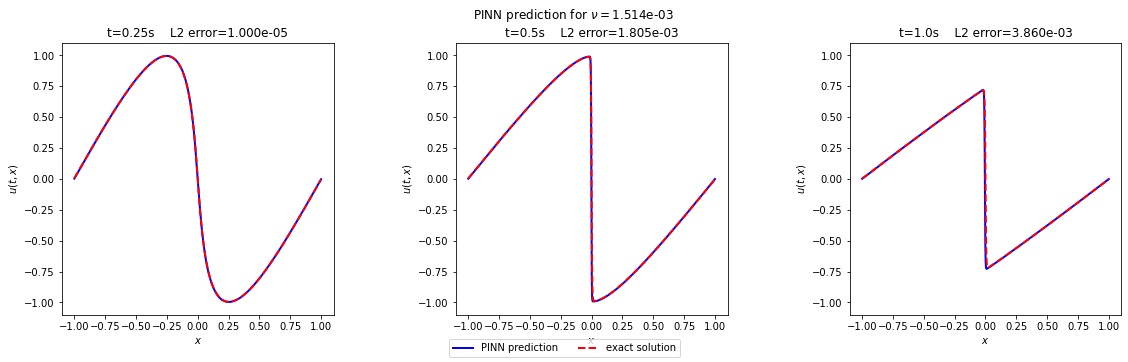
\includegraphics[width=.49\textwidth, height=0.4\textwidth, keepaspectratio]{img/burgers_multi4.png}
        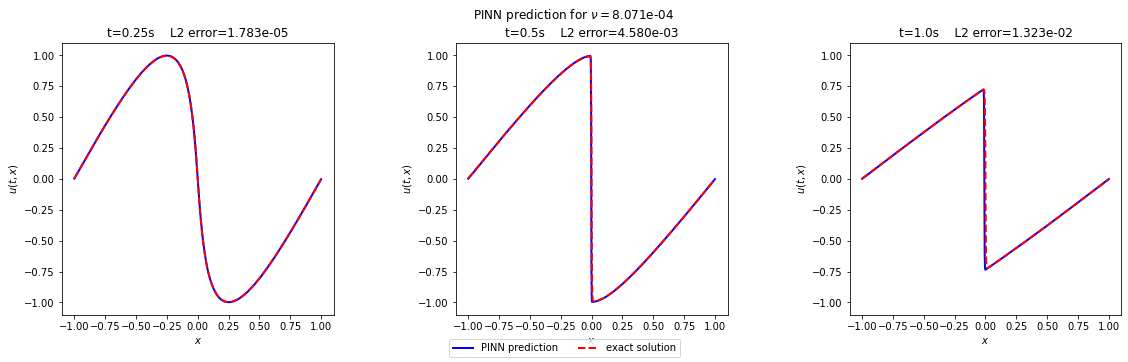
\includegraphics[width=.49\textwidth, height=0.4\textwidth, keepaspectratio]{img/burgers_multi5.png}
        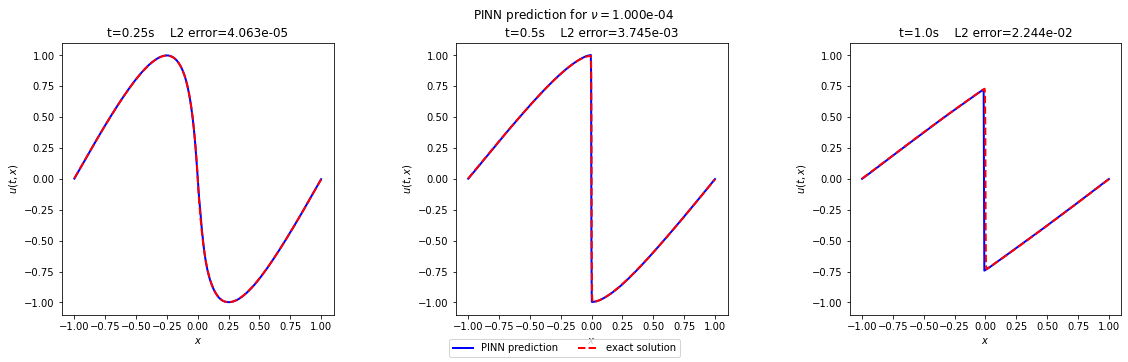
\includegraphics[width=.49\textwidth, height=0.4\textwidth, keepaspectratio]{img/burgers_multi6.png}
    \end{center}
    
\end{frame}


\begin{frame}
    \frametitle{Equation de Burgers en 2D}

    2ème cas test : $\Omega = [0,1.5]\times[0,1]\times[0,1]$ et un paramètre de viscosité $\nu$
    $$
    \begin{cases}
        \partial_t u + \frac{1}{2}\partial_x u^2  + \partial_y u = \nu \Delta u \quad \text{ sur } \Omega\\
        u(0,x,y) = 1.5-2x \quad \forall x \in [-1,1]\\
        u(t,0,y) = 1.5, u(t,1,y) = -0.5, u(t,x,0) = 1.5-2x
    \end{cases}
    $$
\end{frame}

\begin{frame}
    \frametitle{Résultats numérique : $\nu  = 10^{-3}$}
    Avec un réseaux de taille 8x150, après 4h d'entrainements
    \begin{center}
        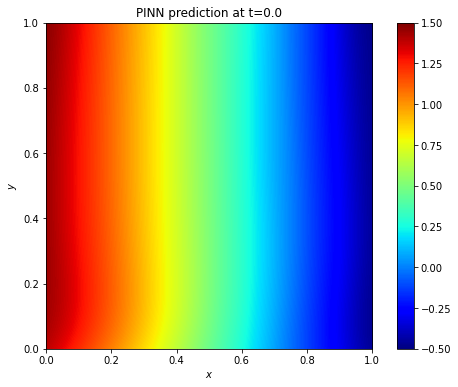
\includegraphics[width=.35\textwidth, height=0.4\textwidth, keepaspectratio]{img/adv_t0.png}
        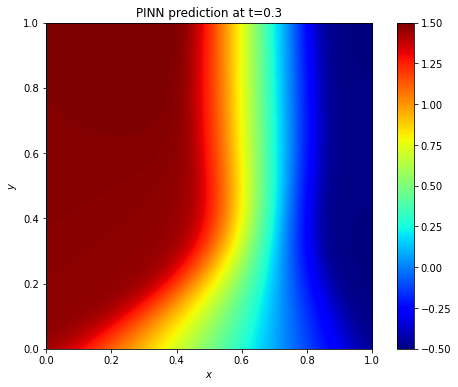
\includegraphics[width=.35\textwidth, height=0.4\textwidth, keepaspectratio]{img/adv_t3.png}
        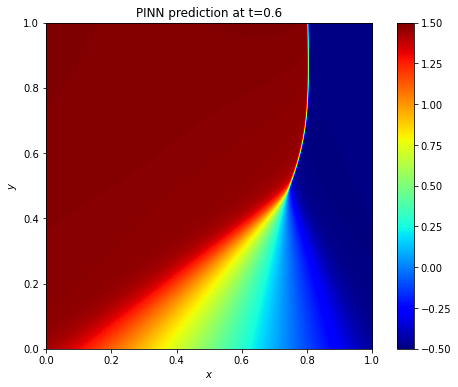
\includegraphics[width=.35\textwidth, height=0.4\textwidth, keepaspectratio]{img/adv_t6.png}
        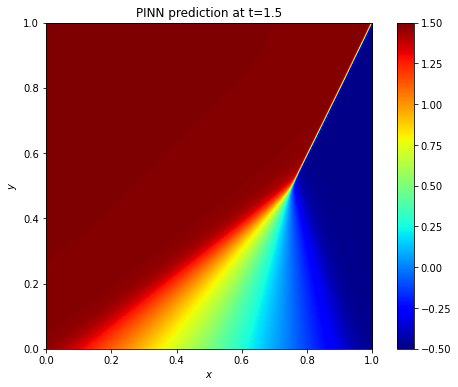
\includegraphics[width=.35\textwidth, height=0.4\textwidth, keepaspectratio]{img/adv_t15.png}
    \end{center}

\end{frame}

\begin{frame}

    \begin{columns}
        \begin{column}{0.5\textwidth}
            \vspace{-0.5cm}
            \begin{center}
                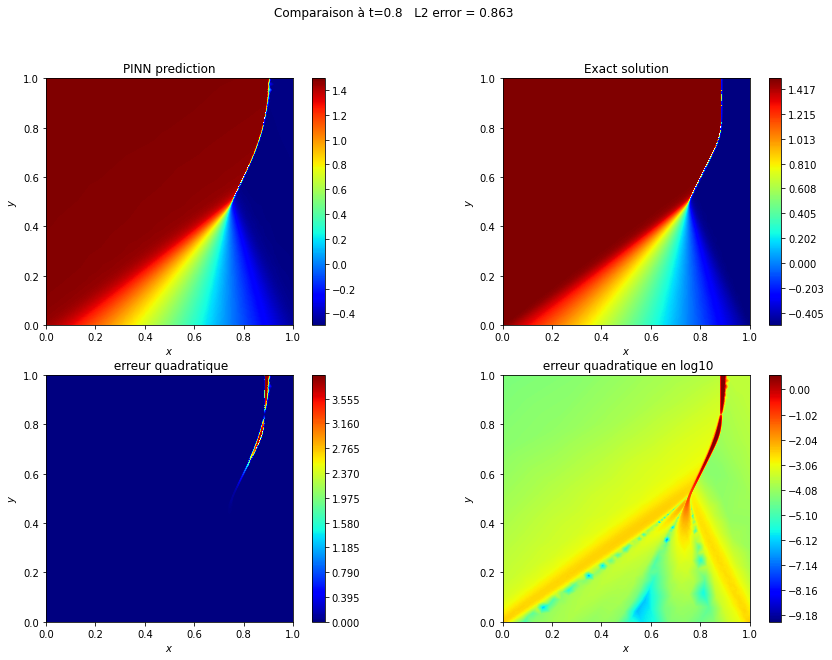
\includegraphics[width=1.\textwidth, keepaspectratio]{img/adv_error2.png}
            \end{center}
        \end{column}
        \begin{column}{0.5\textwidth}  %%<--- here
            \vspace{-0.5cm}
            \begin{center}
                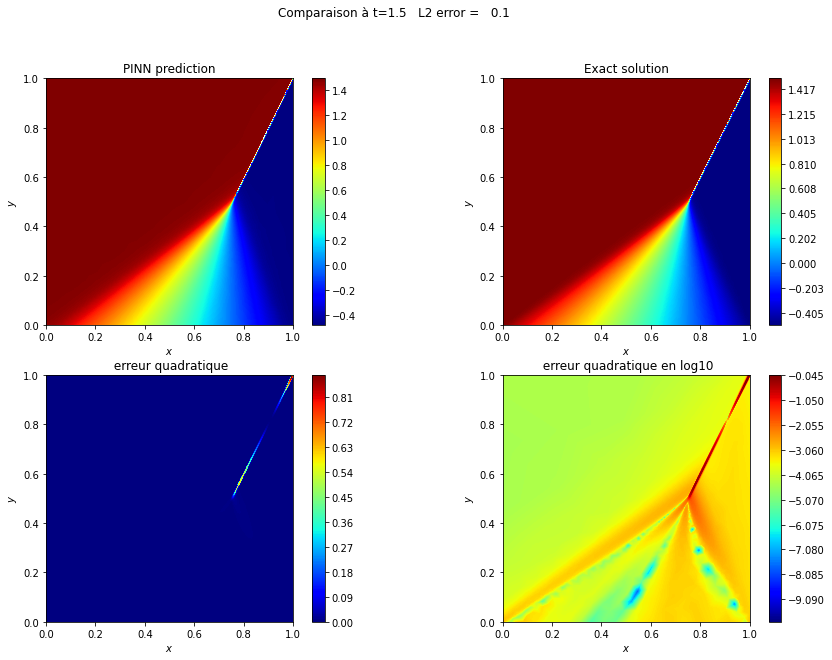
\includegraphics[width=1.\textwidth, keepaspectratio]{img/adv_error.png}
            \end{center}
        \end{column}
        \end{columns}

    \begin{center}
        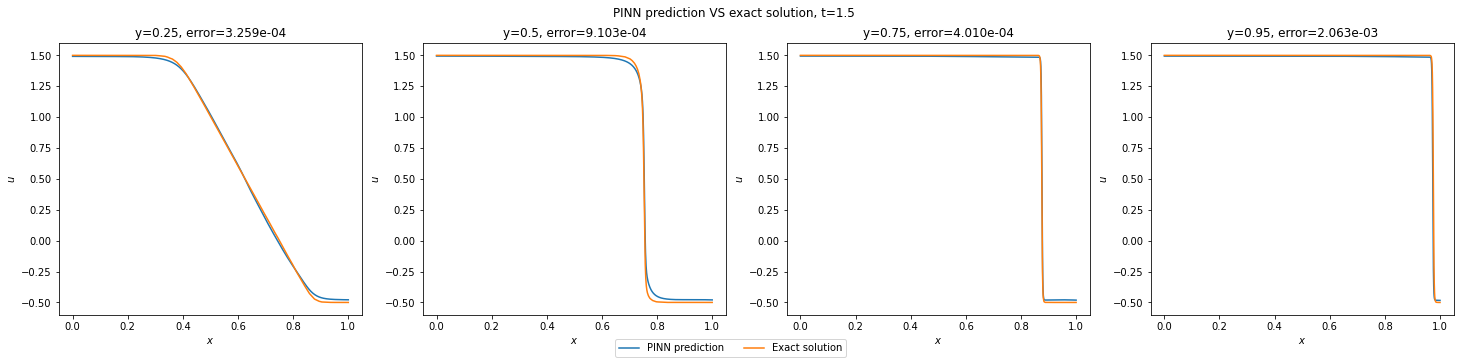
\includegraphics[width=.8\textwidth, height=0.4\textwidth, keepaspectratio]{img/adv_slice.png}
    \end{center}

\end{frame}


\begin{frame}
    \frametitle{Et enfin, la MHD}

    MHD = magnétohydrodynamique =  dynamique des fluides conducteur du courant électrique en présence de champs électromagnétiques (plasmas)

    $$
\begin{cases}
    \partial_t \rho+ \nabla \cdot (\rho V)= 0 \\
    \partial_t V + (V \cdot \nabla)V = \frac{J\times B - \nabla P}{\rho} + \nu\Delta V \\
    \partial_t B = \nabla \times (V\times B - J) \\
    \partial_t P + V\cdot \nabla P = -\Gamma P \nabla\cdot V
\end{cases}
$$
avec $J = \nabla \times B$ et $\nabla \cdot B = 0$

   
\end{frame}

\begin{frame}
    \frametitle{MHD réduite}

    Fluide incompréssible, 2D, avec viscosité $\nu$ et résistivité $\eta$ uniformes

$$
\begin{cases}
    \partial_t \omega + (V \cdot \nabla) \omega = (B \cdot \nabla)J + \nu\Delta \omega \\
    \partial_t \psi + (V \cdot \nabla)\psi = \eta \Delta \psi \\
    \Delta \phi = - \omega \\
    \Delta \psi = - J
\end{cases}
$$
\end{frame}



\begin{frame}
    \frametitle{Instabilité de tilt}

    Configuration d'équilibre intiale : 

    \begin{equation*}
        J_e(x,y) = \begin{cases}
            0 & \text{si r} > 1\\
            -\frac{2k}{j_0(k)}j_1(kr)\frac{y}{r} & \text{si r} \leq 1
        \end{cases}
    \quad \quad 
        \psi_e(x,y) = \begin{cases}
            (\frac{1}{r}-r)\frac{y}{r} & \text{si r} > 1\\
            -\frac{2}{kj_0(k)}j_1(kr)\frac{y}{r} & \text{si r} \leq 1
        \end{cases}
    \end{equation*}

    avec $r=\sqrt{x^2+y^2}$, $j_0$ et $j_1$ les première et seconde fonctions de Bessel de première espèce et $k=3.83170597$

    \begin{center}
        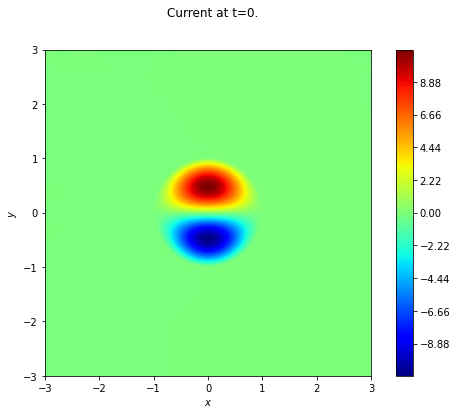
\includegraphics[width=.3\textwidth, height=0.4\textwidth, keepaspectratio]{img/tilt0.png}
        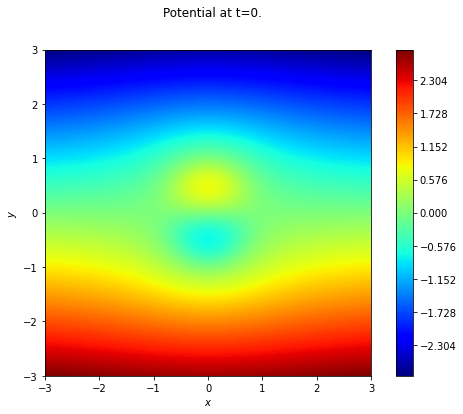
\includegraphics[width=.3\textwidth, height=0.4\textwidth, keepaspectratio]{img/tiltpsi0.png}
    \end{center}

    et $\omega_e = \phi_e = 0$

\end{frame}


\begin{frame}
    \frametitle{Instabilité de tilt}


    \begin{center}
        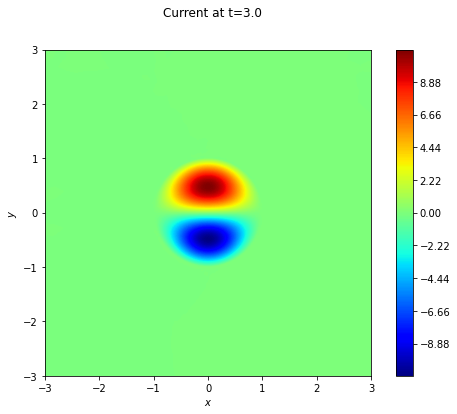
\includegraphics[width=.3\textwidth, height=0.4\textwidth, keepaspectratio]{img/tilt3.png}
        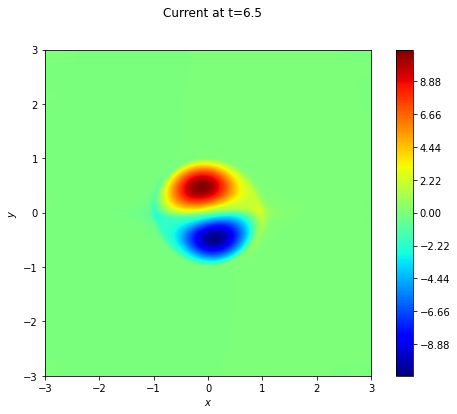
\includegraphics[width=.3\textwidth, height=0.4\textwidth, keepaspectratio]{img/tilt6.png}
        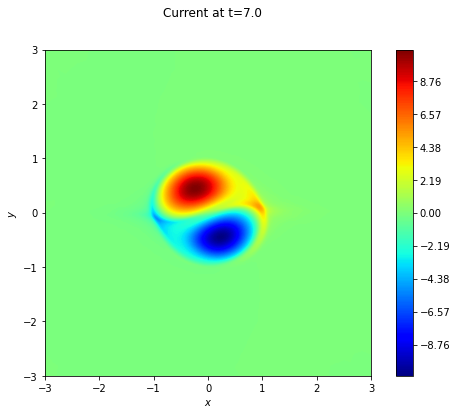
\includegraphics[width=.3\textwidth, height=0.4\textwidth, keepaspectratio]{img/tilt7.png}
        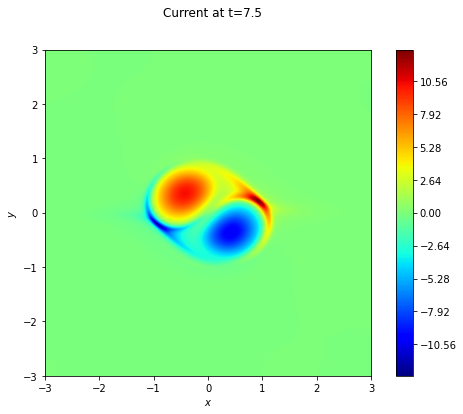
\includegraphics[width=.3\textwidth, height=0.4\textwidth, keepaspectratio]{img/tilt75.png}
        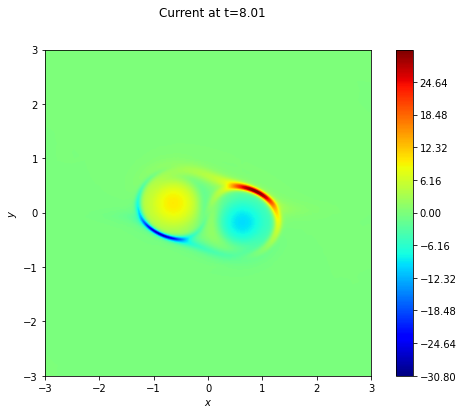
\includegraphics[width=.3\textwidth, height=0.4\textwidth, keepaspectratio]{img/tilt8.png}
        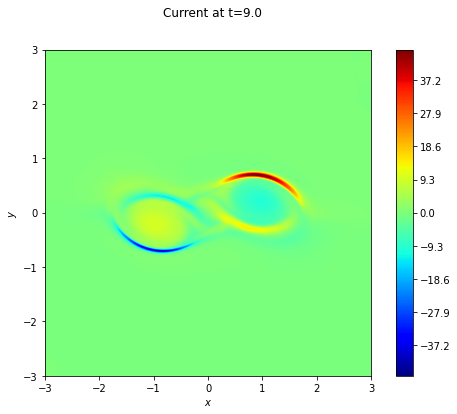
\includegraphics[width=.3\textwidth, height=0.4\textwidth, keepaspectratio]{img/tilt9.png}
    \end{center}

\end{frame}


\nocite{*}
\begin{frame}
    \frametitle{Bibliographie}

    \bibliographystyle{amsalpha}
    {\footnotesize
    \bibliography{diapo}}

\end{frame}


\end{document}